\chapter{State of the Art}

Text goes here.

Focus on multiprocessing models which focus on performance improvements.

\begin{itemize}
    \item Single source kernel: OpenCL, HIP.
    \item Language extensions for high level parallelism: OpenMP, OpenACC, SYCL, C++ AMP.
    \item Proprietary solutions: CUDA.
\end{itemize}

Other types of models which focus on scalability, but not covered \cite{survey_programming_models}:

\begin{itemize}
    \item Actor model
    \item MPI
\end{itemize}

Section \ref{sect:history-gpgpu} covers the history of advancements in GPGPU technology and is based on \cite{brief_history_gpgpu}, a talk by NVIDIA Software Engineer Mark Harris. 

% TODO somewhere around here?
Today, over six hundred applications utilize GPU acceleration across a broad range of industries including: finance, design for manufacturing/construction, artificial intelligence, medical imaging and more.

\section{The History of GPGPU} \label{sect:history-gpgpu}

\subsection{Inception}
The first documented case of computation on a graphics processor dates to June 1985, when Tim Van Hook implemented the world's first GPU ray-tracing on the Ikonas RDS-3000 \cite{ikonas}. Van Hook followed this up the next year with a paper on solid modelling with the Ikonas \cite{solid_modeling_ikonas}.

In August 1999, Kedem et al. \cite{unix_passwords_gpgpu} published a paper where they used experimental graphics engine PixelFlow to perform a brute force attack on Unix passwords. PixelFlow was a heterogeneous parallel machine used for high-speed and high-quality image generation. For their research, PixelFlow was setup with 18 SIMD arrays, each one with 8K processing elements (PE) for a total of 144K (147,456) PEs running at 100Mhz. The machine had some performance problems for this application due to the limited instruction set, which was focused on image computations. Due to this, the results were poorer than expected. It was calculated that the machine would be able to check all lowercase passwords (28.9\% of passwords at the time) in 3.19 hours.

\begin{figure}[h]
    \centering
    
\includegraphics[width=0.5\textwidth]{img/voronoi.png}
    \captionsetup{justification=centering}
    \caption{Generalized Voronoi diagram computed interactively on PC (Credit: Hoff et al.)}
\end{figure}

Also in 1999, Hoff et al. \cite{voronoi_diagrams_gpgpu} managed to perform computations of generalized Voronoi diagrams using graphics accelerators, such as the NVIDIA TNT2, connected to a PC \cite{brief_history_gpgpu}, as opposed to the specialized hardware in the PixelFlow. This was achieved by using the OpenGL API \cite{opengl}. However, at that time GPUs were not programmable. The hardware exposed what is known as a Fixed Function Pipeline which the user could configure according to their needs. With that configuration, the GPU would execute a series of built in math functions which were focused on rendering, not on computation \cite{opengl_fixed_function_pipeline}.

\subsection{Programmable GPUs}
Programmable GPUs did not come until 2001, as NVIDIA introduced GeForce series 3. This replaced the fixed functions in the previous model with programmable shaders which could be controlled by the developers \cite{nvidia_nfinitefx_pixel, nvidia_nfinitefx_vertex}. These features were, of course, aimed at game developers and 3D designers, but they also allowed for new applications of GPU technology.

Using a GeForce 3, Larsen and McAllister achieved the first matrix multiplication done on a GPU \cite{early_matrix_multiplication_gpgpu}. Their work had to be done by mapping the matrices into textures that could be manipulated with the OpenGL API. This textures would be transferred to the GPU, rendered and then copied back to CPU memory to be mapped again to a matrix format so results could be read. Incidentally, the resulting "matrix texture" would be shown on screen. There is no explicit mention of the use of programmable shaders in this work, however this would not have changed the study drastically as the fixed functions of the previous model could handle the operations required. The main problem Larsen and McAllister found was the 8 bit fixed point precision and saturation arithmetic used by the hardware. Saturation arithmetic, although very useful in graphics, makes it harder to design a higher precision fixed-point implementation.

Approximate simulations of natural phenomena were achieved on the GPU by Harris et al. \cite {physics_simulations_gpgpu}. This included interactive visualizations of convection, reaction-diffusion and boiling. As the end effect of the simulation was to display visuals, this application had the advantage that data did not need to be transferred back to the CPU once results were computed. Again, during these experiments the most problematic aspect was the precision of the fixed-point operations. This contributed to more difficult programmability and arithmetic errors. During this work, the researchers exploited the programming capabilities of the GeForce 3 and, at the time, newly released GeForce 4. ATI had also released a programmable GPU in the form of the Radeon 8500, which promised to add more power to the simulations, however the system was not ported to it at the time of publication. 

In late 2002, after seeing the growing trend in general purpose computation on GPUs, Harris coined the term GPGPU, an acronym for "General Purpose computing on Graphics Processing Units" \cite{brief_history_gpgpu}. GPGPU.org, a website dedicated to news and resources on GPGPU research, would go live August 2003.

DirectX 9 (DX9) introduced the Shader Model 2.0 and with it support for floating-point operations. In July 2002, ATI released the first DirectX 9 capable graphics card in the form of the Radeon 9700 PRO \cite{ati_9700_pro}. NVIDIA followed up with their own DX9 GPU, the GeForceFX, in January 2003 \cite{geforcefx}. 

DX9 Hardware allowed researchers to implement algorithms which previously could not be ran on the GPU due to lack of floating-point support. One example of this is global illumination. In \cite{photon_mapping_gpgpu}, Purcell et al. achieve interactive frame rates on a GeForce FX 5900 computing global illumination via photon mapping. This is done by utilizing an incremental approach, where increasingly better approximations are rendered until the image converges, the initial approximations can be shown to the user for interactive feedback. On a 160 x 160 window, it is possible to interactively manipulate the camera, scene geometry and light source. Once interaction stops, the illumination converges in one or two seconds, an example can be seen in figure \ref{fig:lighting-approximations}. 

\begin{figure}[ht] 
    \centering
    \begin{tabular}{ccc}
      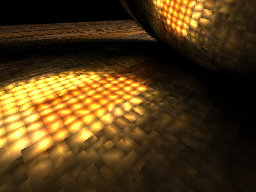
\includegraphics[width=0.3\textwidth]{img/half-second-glass-ball.png} & 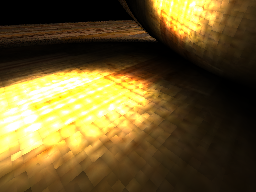
\includegraphics[width=0.3\textwidth]{img/one-second-glass-ball.png} & 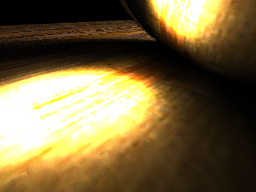
\includegraphics[width=0.3\textwidth]{img/two-second-glass-ball.png} \\
    (a) 0.5s & (b) 1.0s & (c) 2.0s
    \end{tabular}
    \captionsetup{justification=centering}
    \caption{Lighting approximations over time (Credit: Purcell et al.)}
    \label{fig:lighting-approximations}
\end{figure}

The main bottleneck that Purcell et al. faced in their paper stemmed from the lack of random access writes. While the original photon mapping algorithm uses a balanced k-d tree, it is not possible to construct one on the GPU due to this limitation. Instead, the researchers had to modify the algorithm in order to account for this, replacing the k-d tree with a uniform grid. To build this grid, they implemented two algorithms, bitonic merge sort and stencil routing. The bitonic sort is computationally less efficient, needing \(O(\log^2 n)\) rendering passes. On the other hand stencil routing can be computed in a single pass but suffers from memory readback performance bottlenecks. 

All the kernels were written in Cg, a general purpose language for GPUs released by NVIDIA at the start of 2003 \cite{nvidia_cg}. The design of Cg was inspired by the C language to provide a high level language that is still close to the underlying hardware. The syntax of C served as a starting point which was then extended and modified as necessary to support GPU architectures effectively. The general purpose nature of the language allows the programmer to use very similar code to program the vertex and fragment stages of the rendering pipeline. This also simplifies programming for GPGPU applications, an aspect that was taken into account when designing the language due to the rising popularity of the field.

\subsection{Brook}
Languages like Cg, Microsoft's HLSL and OpenGL's GLslang allowed for shaders to be written in C-like syntax. However, they still required the programmer to express GPU applications in terms of graphics primitives and to use the existing graphics APIs to control the rest of the graphics pipeline, such as memory allocation and loading programs. In August 2004 researchers at Stanford University present Brook \cite{brook}, a programming environment that provides developers with a view of the GPU as a streaming coprocessor.

Instead of working with textures and shaders, the Brook language allows the programmer to think in terms of streams and kernels. A stream is a collection of records (elements) and is denoted by angle-brackets, i.e. \texttt{float x<100>}. Access to streams is limited to kernels and the \texttt{streamRead} and \texttt{streamWrite} operators, which transfer memory between memory and streams. A kernel is a function that performs parallel operations over one or more streams. Calling a kernel on a stream performs an implicit loop over the elements of the stream, invoking the body of the kernel for each element. An example Brook snippet can be seen below.

\begin{lstlisting}[style=BrookStyle, caption=Brook saxpy example]
kernel void saxpy(float a, float4 x<>, float4 y<>, out float4 result<>) {
    result = a*x + y;
}

void main(void) {
    float a;
    float4 X[100], Y[100], Result[100];
    float4 x<100>, y<100>, result<100>;
    // ... initialize a, X, Y ...
    streamRead(x, X);               // copy data from mem to stream
    streamRead(y, Y);
    saxpy(a, x, y, result);         // execute kernel on all elements
    streamWrite(result, Result);    // copy data from stream to mem
}   
\end{lstlisting}

A kernel accepts different types of arguments:

\begin{itemize}
    \item Input streams that contain read-only data for kernel processing.
    \item Output streams (marked with the \texttt{out} keyword) that store the result of a kernel computation.
    \item Gather streams which are declared as a C array with brackets, i.e. \texttt{gather[]}. A gather stream allows for arbitrary indexing of its elements.
    \item Non-stream arguments, which are read-only constants.
\end{itemize}

Due to the same GPU limitations experienced by Purcell et al., Brook does not provide arbitrary writes, only arbitrary reads with the gather streams.

The Brook compilation and runtime system maps the language onto existing programmable GPU APIs, including OpenGL and DirectX. The system consists of two components: \texttt{brcc}, a source-to-source compiler and the Brook Runtime (BRT), a library that provides runtime support for kernel execution. \texttt{brcc} maps Brook kernels into Cg shaders which are then translated into GPU assembly by vendor-provided shader compilers. Additionally, it emits C++ code which uses BRT to invoke the kernels. 

\subsection{The Unified Shader Model}

In November 2005, Microsoft launched the XBOX 360 console. A noteworthy aspect of this launch is that the console used the first unified shader architecture GPU on the market, the ATI Xenos \cite{xbox_360_specs}. Previously, GPUs had different processing units which either handled vertex or fragment shader operations. In the unified shader model, there is a single type of unit, called shader core, which can handle both type of operations. The main selling point of this change is that greater flexibility allowed for all the units to be used during rendering, no matter the type of workload. With the classical fixed shader model, heavy polygon scenes would leave the fragment units idle, while heavy pixel scenes would underutilize the vertex units. This issue is illustrated in figure \ref{fig:gpu-fixed-shader-perf}. Figure \ref{fig:gpu-unified-shader-perf} shows how the unified shader model is able to better utilize the available resources.

\begin{figure}[ht]
    \centering
    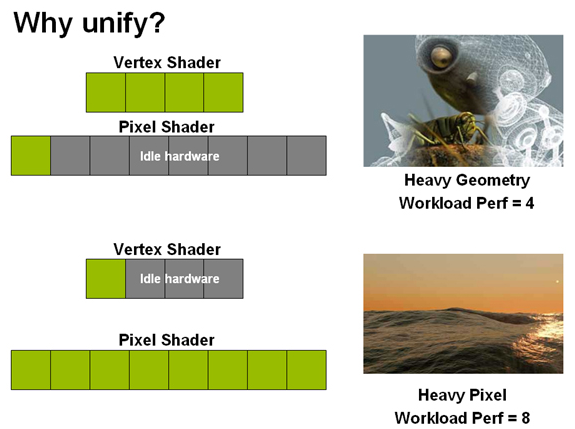
\includegraphics[width=0.6\textwidth]{img/classic-model-gpu-idle-units.png}
    \captionsetup{justification=centering}
    \caption{Fixed shader model performance characteristics (Credit: NVIDIA)}
    \label{fig:gpu-fixed-shader-perf}
\end{figure}

\begin{figure}[ht]
    \centering
    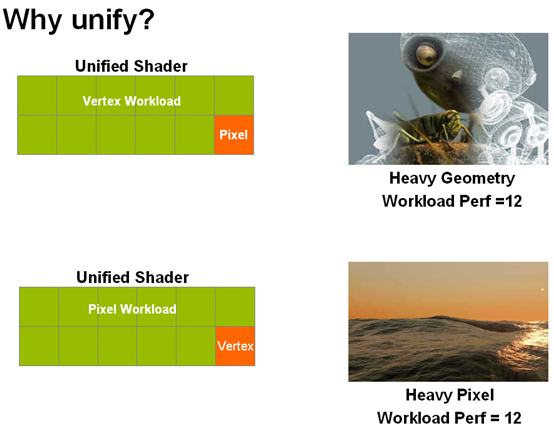
\includegraphics[width=0.6\textwidth]{img/unified-shader-gpu-utilization.png}
    \captionsetup{justification=centering}
    \caption{Unified shader performance characteristics (Credit: NVIDIA)}
    \label{fig:gpu-unified-shader-perf}
\end{figure}

While ATI produced the first unified shader GPU for the XBOX 360, NVIDIA was the one  to release the model in PCs with the GeForce 8800 in November 2006. DirectX 10 had introduced Shader Model 4.0 which included a unified shader instruction set. Even though a unified architecture was not a requirement to use DirectX 10, it provided better efficiency, load-balancing and power utilization \cite{geforce_8800_architecture}. A block diagram of the GeForce 8800 can be seen in figure \ref{fig:8800-arch}. The streaming processors (SP) marked in green are the units in charge of all the shader processing (the shader cores).

\begin{figure}[ht]
    \centering
    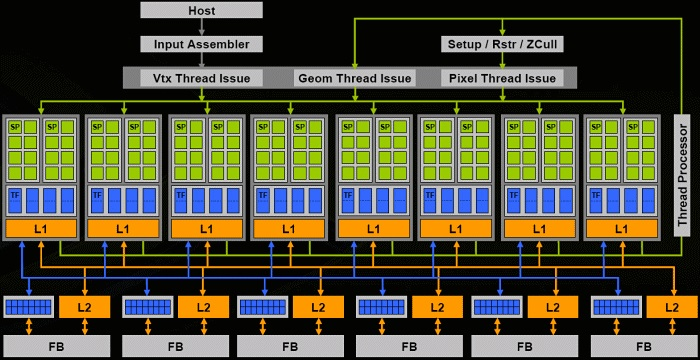
\includegraphics[width=\textwidth]{img/geforce-8800-block-diagram.png}
    \captionsetup{justification=centering}
    \caption{GeForce 8800 GTX Block Diagram (Credit: NVIDIA)}
    \label{fig:8800-arch}
\end{figure}

\subsection{GPGPU Vendor Support}

ATI (from here on out referred to as AMD due to their acquisition in 2006) was also the first vendor to release direct support for GPGPU with its CTM or "Close to To The Metal" system in late 2006. CTM provides raw assembly level access with its hardware abstraction layer (HAL). The compute abstraction layer (CAL) adds higher level constructs and a C API, however this only covers context, memory management and kernel execution, the kernel itself must still be written in a low level AMD intermediate representation \cite{amd_ctm_programming_guide}. For higher level programming, AMD also supported compilation of Brook programs directly to the hardware \cite{gpu_computing}.

By providing a first party computing model, CTM eliminates the need for developers to work with graphics APIs and deal with a rendering pipeline. Instead of having to adapt algorithms work with textures, vertices, pixels and shaders, the developer can perform computation by binding memory as inputs and outputs to the stream processors directly. This includes Brook, which no longer has the requirement to work on top of a graphics API backend.

In June of 2007, NVIDIA introduced CUDA \cite{cuda_toolkit_archive}. The significant redesign that came with the adoption of unified shaders for the GeForce 8800 GTX, as well as the flexibility achieved by the final model, allowed NVIDIA to develop a hardware and software solution for data-intensive computing. 

The CUDA C++ language which is a minimal extension over C++ adding parallelism features. As opposed to AMD CTM, which combined the CAL C API with a low level kernel language, this programming model is single source. CPU (host) code and GPU (kernel) code are written in the same language and can be contained in the same file. 

CUDA is a higher level interface than AMD's CAL, but it also provides more hardware access than Brook. In exchange for requiring more hardware knowledge, CUDA exposes multiple levels of memory hierarchy, per-thread registers, fast shared memory between threads in a block, board memory and host memory. In addition, while Brook only exposes a single dimension of parallelism, data parallelism via streaming, CUDA provides data parallelism and multithreading. CUDA kernels are also more flexible, as they allow the use of pointers, arbitrary writes and thread synchronization between threads in a single block \cite{gpu_computing}.

Overall, CUDA's advantages over AMD's CTM gave NVIDIA the upper hand in the GPGPU field and it is still in use to this day. By contrast, in 2008, AMD's CTO of graphics announced that the company was shifting its focus away from CTM and into the upcoming OpenCL standard \cite{amd_ctm_ditch}, detailed in the following section.

\section{OpenCL}

Released in December 2008, Open Compute Language or OpenCL \cite{opencl_spec} is an open industry standard for programming a heterogeneous collection of CPUs, GPUs and other discrete computing devices organized into a single platform. It provides a framework for parallel programming and includes a language, API, libraries and a runtime system to support software development. By leveraging OpenCL, an application can use a host and one or more OpenCL devices as a single heterogeneous parallel computer system.

The framework is comprised by the following components:
\begin{itemize}
    \item \textbf{Platform layer}: allows the host program to create contexts and discover OpenCL devices and their capabilities.
    \item \textbf{Runtime}: allows the host program to manipulate contexts one they have been created.
    \item \textbf{Compiler}: creates program executables that contain OpenCL kernels. Depending on the capabilities of a device, the compiler may build executables from either OpenCL C source strings, the SPIR-V intermediate language, or device-specific program binary objects. Some implementations may support other kernel languages or intermediate languages.
\end{itemize}

OpenCL C \cite{opencl_c_spec} is the programming language provided by the standard to write kernels that execute on an OpenCL device. OpenCL C is based on the \textit{ISO/IEC 9899:1999 - Programming languages - C} specification (also referred to as C99) \cite{c99}, with the addition of some \textit{ISO/IEC 9899:2011 - Information technology - Programming languages - C} specification (also referred to as C11) \cite{c11} features, plus some extensions and restrictions to support parallel kernels.

This dedicated kernel language allows the developer to write a single kernel code base and execute it in different devices. This ensures the \textit{functional} portability of code across devices, eliminating the need for applications to be re-coded on a per-device or per-programming toolkit basis \cite{performance_portability_2013}. However, portability issues may still arise if the hardware supports different versions of the standard. In addition, there can also be issues in terms of performance portability due to architecture differences and compiler optimizations available on each platform \cite{performance_portability_2013, performance_portability_2019, performance_portability_2020}. For maximum performance, some tweaking of the source code may still be necessary depending on which device is being targeted \cite{optimizing_opencl_fpga_integer, optimizing_opencl_fpga_automata}.

SPIR-V is an intermediate language which is also supported as an input language for OpenCL. Instead of distributing and ingesting OpenCL C in the host, developers can precompile their kernels into SPIR-V, allowing for faster kernel load times and avoiding directly exposed source code \cite{spir_overview}. While SPIR-V is also supported by the Vulkan \cite{vulkan} graphics API, it uses a different execution mode of the language (\textbf{GLCompute} versus \textbf{Kernel} for OpenCL), so compute codes are not interchangeable \cite{spir_spec}. Another caveat is that SPIR-V support is only mandatory for OpenCL 2.1 and 2.2 devices, support was made optional for OpenCL 3.0 devices \cite{opencl_spec}.

Today, OpenCL is at the forefront of heterogeneous architecture programming. Seventeen different companies (including Apple, Intel, AMD and NVIDIA) distribute products conforming to the standard \cite{opencl_conformant_companies}. This allows an OpenCL kernel to run on the majority of hardware available on the market, including CPUs, GPUs, FPGAs and more.

\begin{figure}[ht]
    \centering
    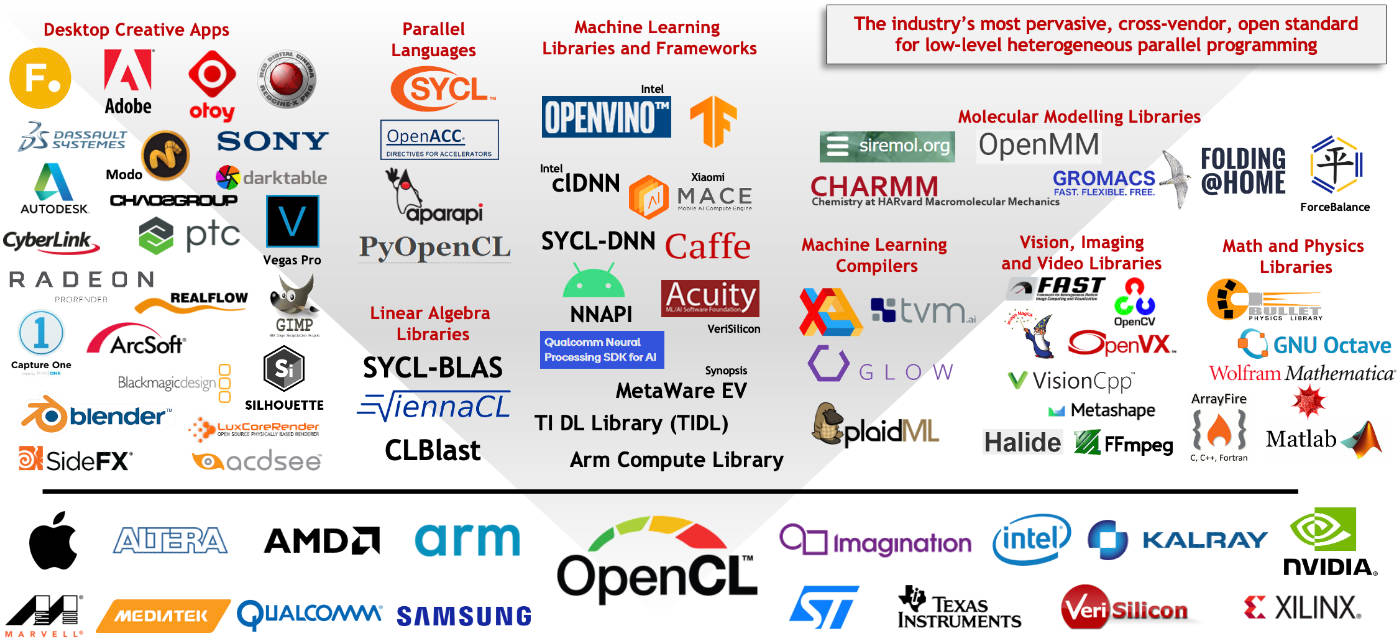
\includegraphics[width=\textwidth]{img/opencl-accelerated-apps.png}
    \captionsetup{justification=centering}
    \caption{OpenCL accelerated applications (Credit: Khronos Group)}
\end{figure}

Due to its popularity, a significant amount papers have been published looking into different types of extensions on the framework. We will focus on the extensions that are particularly relevant to our work. Section \ref{sub-sect:abstraction-layers} covers abstraction layers on top of OpenCL and section \ref{sub-sect:kernel_scheduling} covers kernel scheduling algorithms.

\subsection{Abstraction Layers} \label{sub-sect:abstraction-layers}
Even though OpenCL simplifies a big part of heterogeneous systems programming by providing a common API across devices, it still is a complex task. 
The articles presented in this section focus on simplifying the problem further by adding an abstraction layer on top of OpenCL.

In EngineCL \cite{enginecl}, a new object-oriented API is introduced. The EngineCL class provides a higher level view of the OpenCL context and management of the available devices. The engine in turn uses a Program object which internally manages all the data transfers between the device buffers, the user only needs to provide host input and output buffers, as well as the kernel arguments in order to begin execution. In addition, multiple devices can be used during a single run, the scheduling of which is handled by a Scheduler object. Different scheduling strategies are tested by the paper, with the best results achieved by the HGuided algorithm. HGuided is a dynamic algorithm which starts by assigning big block sizes to all devices and reducing the size of subsequent ones as the execution progresses. This reduces data transfer and synchronization overhead while allowing devices to finish simultaneously towards the end of the execution.

A different approach is presented by FluidiCL \cite{fluidicl}, where the OpenCL API is maintained but implemented in such a way that the user can treat multiple devices as a single entity. Thus, it is very easy to adapt an existing OpenCL application to run using FluidiCL, as all function calls are maintained. The paper considers the implementation running on an experimental system with a single GPU and CPU. At the time of setup, both kernel compilation and buffer writes are broadcasted to both devices. That is, the kernel is compiled for both and, likewise, the input data is transferred to the both of their buffers. When the execution starts, the GPU starts running the kernel with a decreasing order of work-group IDs, meanwhile the CPU executes smaller sub-kernels in increasing order of work-group IDs. At some point, when the work-groups IDs handled by both cross over, the work is finished and the results are merged on the GPU.

\subsection{Kernel Scheduling} \label{sub-sect:kernel_scheduling}
Multiple different techniques are discussed in order to optimize the scheduling of the kernels on the devices available on the platform. The overall objective always being minimizing the turnaround time of a kernel or group of kernels.

\cite{transparent_cpu_gpu_collaboration} proposes the SKMD (Single Kernel Multiple Devices) system, where the workload of a single kernel can be split among all the available devices. At runtime, a partitioning algorithm will determine how to make this split, based on memory access pattern analysis of the kernel and previous profiling data. An effective partitioning makes sure that the performance improvements outweigh the overhead of extra memory transfers to the different devices. 

Machine learning is an alternative used to forgo the need of profiling the kernels before scheduling. \cite{smart_multitasking_scheduling} achieves this by implementing a model to predict the kernel speedup on a particular device based on static analysis of the code. Also, instead of focusing on a single kernel, it manages scheduling of multiple kernels, possibly belonging to different applications. A very similar approach is also proposed by \cite{load_balance_model_opencl_integrated_cluster}.

\section{OpenMP \& OpenACC}
In this section we will tackle OpenMP and OpenACC in conjunction as they take very similar approaches.

Both projects are composed of a library and set of compiler directives that provide a model for parallel programming across different architectures. Support is provided for the C, C++ and Fortran languages. The directives extend the languages with useful constructs for parallelizing applications. Further control of the runtime environment is possible through the library \cite{openmp_spec, openacc_spec}.

OpenMP and OpenACC allow for quick adaptation of existing single threaded code into a parallel execution model. This work requires a compiler which supports the standard, meaning that it is able to handle the directives and generate multithreaded code automatically. 

Up until version 4.0, OpenMP only allowed for this code to be compiled for and executed on the CPU. Version 4.0 (2013) introduced offloading of the parallel code to other devices like GPUs or FPGAs \cite{openmp_gpu_support}. Meanwhile OpenACC focused on heterogeneous computing and accelerator offloading from the start \cite{openacc_initial_spec}, also treating the multicore CPU itself as a device.

\cite{openmp_vs_openacc} provides a comparison of both programming models in terms of programmability and expressiveness. Here the authors denote the differences between OpenMP and OpenACC when implementing common parallel programming patterns targeting accelerators. Overall, the resulting code and directives used are mostly equivalent, with OpenACC having a slight advantage thanks to providing accelerator support since its inception. In terms of programmer effort, there is no significant difference. In terms of performance however, \cite{cuda_openacc_openmp_performance} shows that the code generated by OpenACC is able to utilize more memory bandwidth and thus perform better than OpenMP, specially when using a naïve approach. Still, both approaches fall behind a pure CUDA kernel.

Finally, the possibility to use both models at the same time exists. Works like \cite{openmp_openacc_multigpus} exploit parallelism on the CPU with OpenMP to schedule code to run on multiple GPUs. \cite{openmp_openacc_molecular_docking} also leverages this hybrid approach to run kernels which are more GPU friendly on the GPU using OpenACC while running less friendly kernels with OpenMP CPU parallelization. 

\section{SYCL}
SYCL \cite{sycl_2020_standard} is a C++ programming model for heterogeneous computing. It builds on the underlying concepts, portability and flexibility of parallel APIs or standards like OpenCL while adding the ease of use and flexibility of single-source C++. Device and host code live on the same file and can be written in C++ according to the C++17 standard (ISO/IEC 14882:2017 Programming languages — C++) \cite{cpp17} and also the newest C++20 standard (ISO/IEC 14882:2020 Programming languages — C++) \cite{cpp20}. 

For compatibility reasons, the entire set of C++ features is not available in device code. In particular, SYCL device code does not support virtual function calls, function pointers, exceptions, runtime type information and dynamic memory allocation.  This still leaves a big portion of the standard which is compatible with host and device code alike, allowing the reuse of types, library code, templates and abstractions. In addition, the programmer does not need to switch between languages depending which part of the code base they are modifying. It is also important to note that, as long as there is no dependence created with the underlying SYCL implementation, a standard C++ compiler can compile SYCL programs to run directly on the host CPU, without any external accelerator.

To allow for easy integration, SYCL is designed to allow each source file to be passed through multiple different compilers, the outputs of which will be combined into a single source file. The programmer can then add SYCL code to an existing project and continue using their preferred host compiler while the SYCL tools handle compilation for the device code.

An example SYCL code snippet can be seen below. 

\begin{lstlisting}[style=CStyle, caption=SYCL saxpy example]
using namespace sycl;
float A;
float h_X[100], h_Y[100], h_Z[100];

// ... initialize A, h_X, h_Y ...

queue q; // Queue to enqueue work to the default device

// Wrap the arrays in buffers
buffer<float,1> d_X { h_X, range<1>(100) };
buffer<float,1> d_Y { h_Y, range<1>(100) };
buffer<float,1> d_Z { h_Z, range<1>(100) };

q.submit([&](handler& h) {
    auto X = d_X.get_access<access::mode::read>(h);
    auto Y = d_Y.get_access<access::mode::read>(h);
    auto Z = d_Z.get_access<access::mode::read_write>(h);

    // Enqueue a parallel_for task with 100 work-items executing the saxpy kernel
    h.parallel_for(100, [=] (id<1> idx) {
        Z[idx] = A * X[idx] + Y[idx];
    });
});
q.wait();
\end{lstlisting}

The code within the the lambda argument to the \texttt{parallel\_for} is the device kernel. This code will be compiled using the device compiler and executed on the device.

SYCL can be laid out on top of multiple backends. A backend exposes one or multiple SYCL platforms (collections of devices). For example, implementations can expose an OpenCL backend to give access to OpenCL devices, or a CUDA backend to give access to NVIDIA GPUs. Apart from the generic API that all backends must implement in order to provide the basic device functionality, each backend can expose their specific features through interoperability headers to provide the developer with more control at the expense of portability.

When building a SYCL application, the user can choose the backends which will be used. This is the set of \textit{active backends} for the application. The application can then be run on any host platform that supports at least one of the active backends. The subset of active backends which are supported by the host platform at runtime are called the \textit{available backends}.

A diagram with the SYCL implementations in development and their provided backends can be seen in figure \ref{fig:sycl-implementations}. As shown, the available SYCL implementations cover a wide range of hardware. As long as the programmer does not use any backend-specific feature, their application can be executed in any available implementation without modifications.

\begin{figure}[ht]
    \centering
    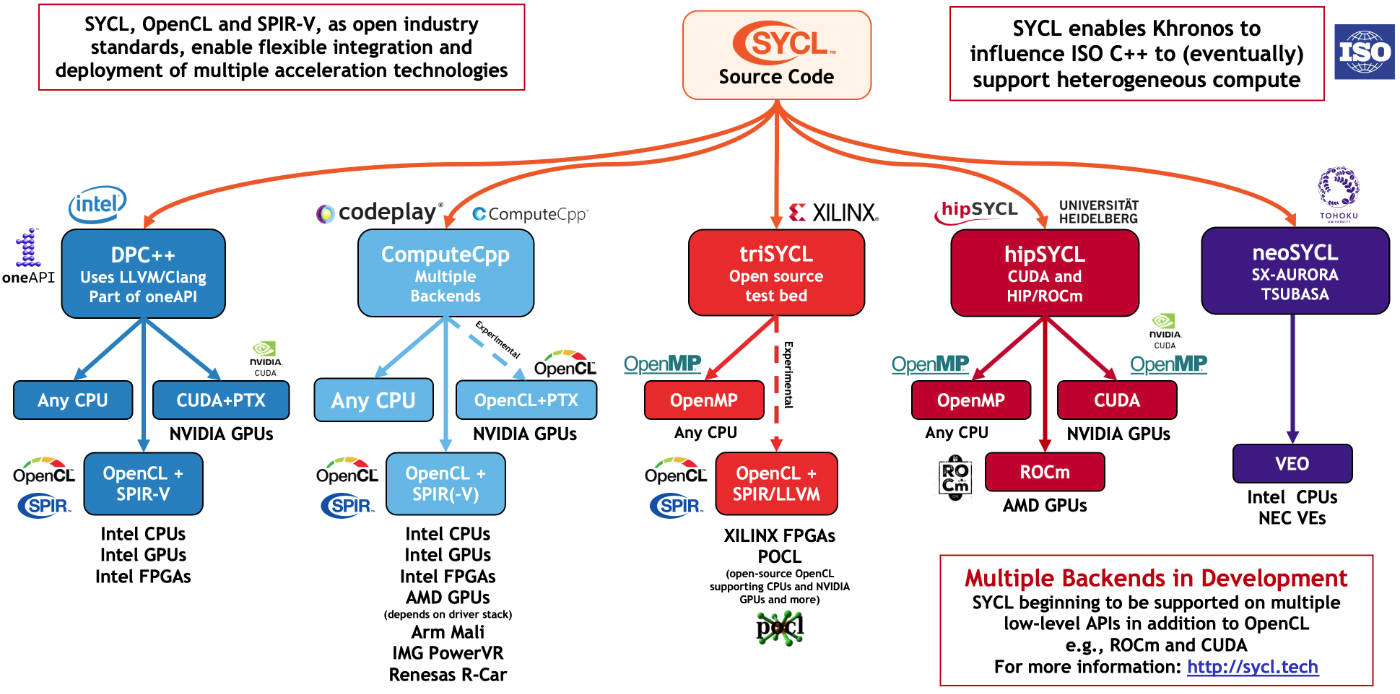
\includegraphics[width=\textwidth]{img/sycl-implementations.png}
    \captionsetup{justification=centering}
    \caption{SYCL implementations in development (Credit: Khronos Group)}
    \label{fig:sycl-implementations}
\end{figure}

\subsection{Celerity}

\section{Kokkos}
\cite{kokkos}

\section{Other Programming Models}

\subsection{AMD ROCm}
AMD ROCm is an open-source software development platform for HPC GPU computing. It is AMD's latest competitor to NVIDIA's CUDA. 

During the 


HIP is a C++ Runtime API and kernel language very similar to CUDA that is portable across NVIDIA and AMD GPUs. It is a part of the AMD ROCm ecosystem, an open source project led by AMD. Supporting both vendors and being open source gives it an advantage over CUDA, however the high level of CUDA adoption has slowed down support for HIP in accelerated applications.

\subsection{C++ AMP}
Appears dead. Stack overflow post by one of the authors \url{https://stackoverflow.com/a/38604348/7983805}

\section{Standalone works}

Here goes what we don't where to put. Also may be deleted entirely.

\subsection{Kernel scheduling}

\cite{dynamic_self_scheduling} presents HDSS, a Heterogeneous Dynamic Self Scheduler, which can reschedule at runtime how the workload is partitioned across the devices. This is achieved by a two phase approach. First, in the adaptive phase, the scheduling algorithm will measure the relative performance across devices by dispatching increasing block sizes. Once an accurate performance approximation for each device is calculated, the completion phase starts. Here the scheduler assigns the largest possible block size to each device, according to its calculated performance, in order to minimize data transfer overhead. The approach presented not only keeps all devices busy during the entire execution, but also fully utilizes them by providing appropriate block sizes. 
